%%%%%%%%%%%%%%%%%%%%%%%%%%%%%%%%%%%%%%%%%%%%
% Chapitre 8
%%%%%%%%%%%%%%%%%%%%%%%%%%%%%%%%%%%%%%%%%%%%

\chapter{Évaluation de la méthode GLM-DT dans un cadre statistique Euclidien}
\label{Chapter8}

Dans ce chapitre, nous allons exposer tous les résultats obtenus, dans le cadre statistique Euclidien,
afin d'évaluer la méthode de détection basée sur les tenseurs développée au cours de la thèse \textit{GLM-DT}.
L'évaluation est composée de trois points principaux.
Tous d'abord, nous allons regarder si l'utilisation du tenseur complet peut être une plus-value 
par rapport aux méthodes classiques basées sur les indices scalaires \textit{GLM-FA} et \textit{GLM-MD}
pour les différents types de lésions simulés.
Ces résultats seront discutés en fonction des études déjà menées dans la littérature.
Ensuite, nous nous intéresserons à savoir si l'utilisation d'informations supplémentaires peut améliorer les performances 
de la méthode \textit{GLM-DT}.\\


% \minitoc

%----------------------------------------------------------------------------------------


\section{Méthodes basées sur les indices scalaires \textit{vs}\\ méthode GLM-DT}

\subsection{Résultats sur données synthétiques}
La \figref{fig:res_scalar} présente que seule la méthode basée tenseur \textit{GLM-DT} est capable de détecter les 4 types de lésions.
En effet, les méthodes basées sur les indices scalaires \textit{GLM-FA} et \textit{GLM-MD} échouent toutes les deux à détecter une modification de l'orientation de la diffusion.
Nous remarquons que les méthodes \textit{GLM-MD} et \textit{GLM-DT} montrent des performances très similaires pour les trois premiers types de lésions 
et que \textit{GLM-FA} est supérieure aux eux autres méthodes pour détecter une augmentation de la diffusion radiale.
En ce qui concerne la modification d'orientation de la diffusion, les méthodes \textit{GLM-FA} et \textit{GLM-MD} présentent des résultats supérieurs à 50\% 
ce qui peut paraître incohérent puisque un changement d'orientation de diffusion n'influe pas sur la géométrie des tenseurs.
Ce comportement peut être expliquer par les pré-traitements appliqués aux images et notament l'étape de filtrage : 
un filtre gaussien va moyenner les tenseurs modifiés avec un voisinage composé de tenseurs non-modifiés ce qui produit des tenseurs de formes différentes, 
et par conséquent, provoque des changements des valeurs de FA et de MD bien qu'ils n'est pas été simulés.

Pour conclure, nous pouvons dire que la méthode \textit{GLM-DT} semble être le meilleur compromit pour détecter tous les types de changements,
bien qu'elle ne surpasse pas clairement les deux autres méthodes pour chaque type de lésion.

\begin{figure*}[t]
    \centering
    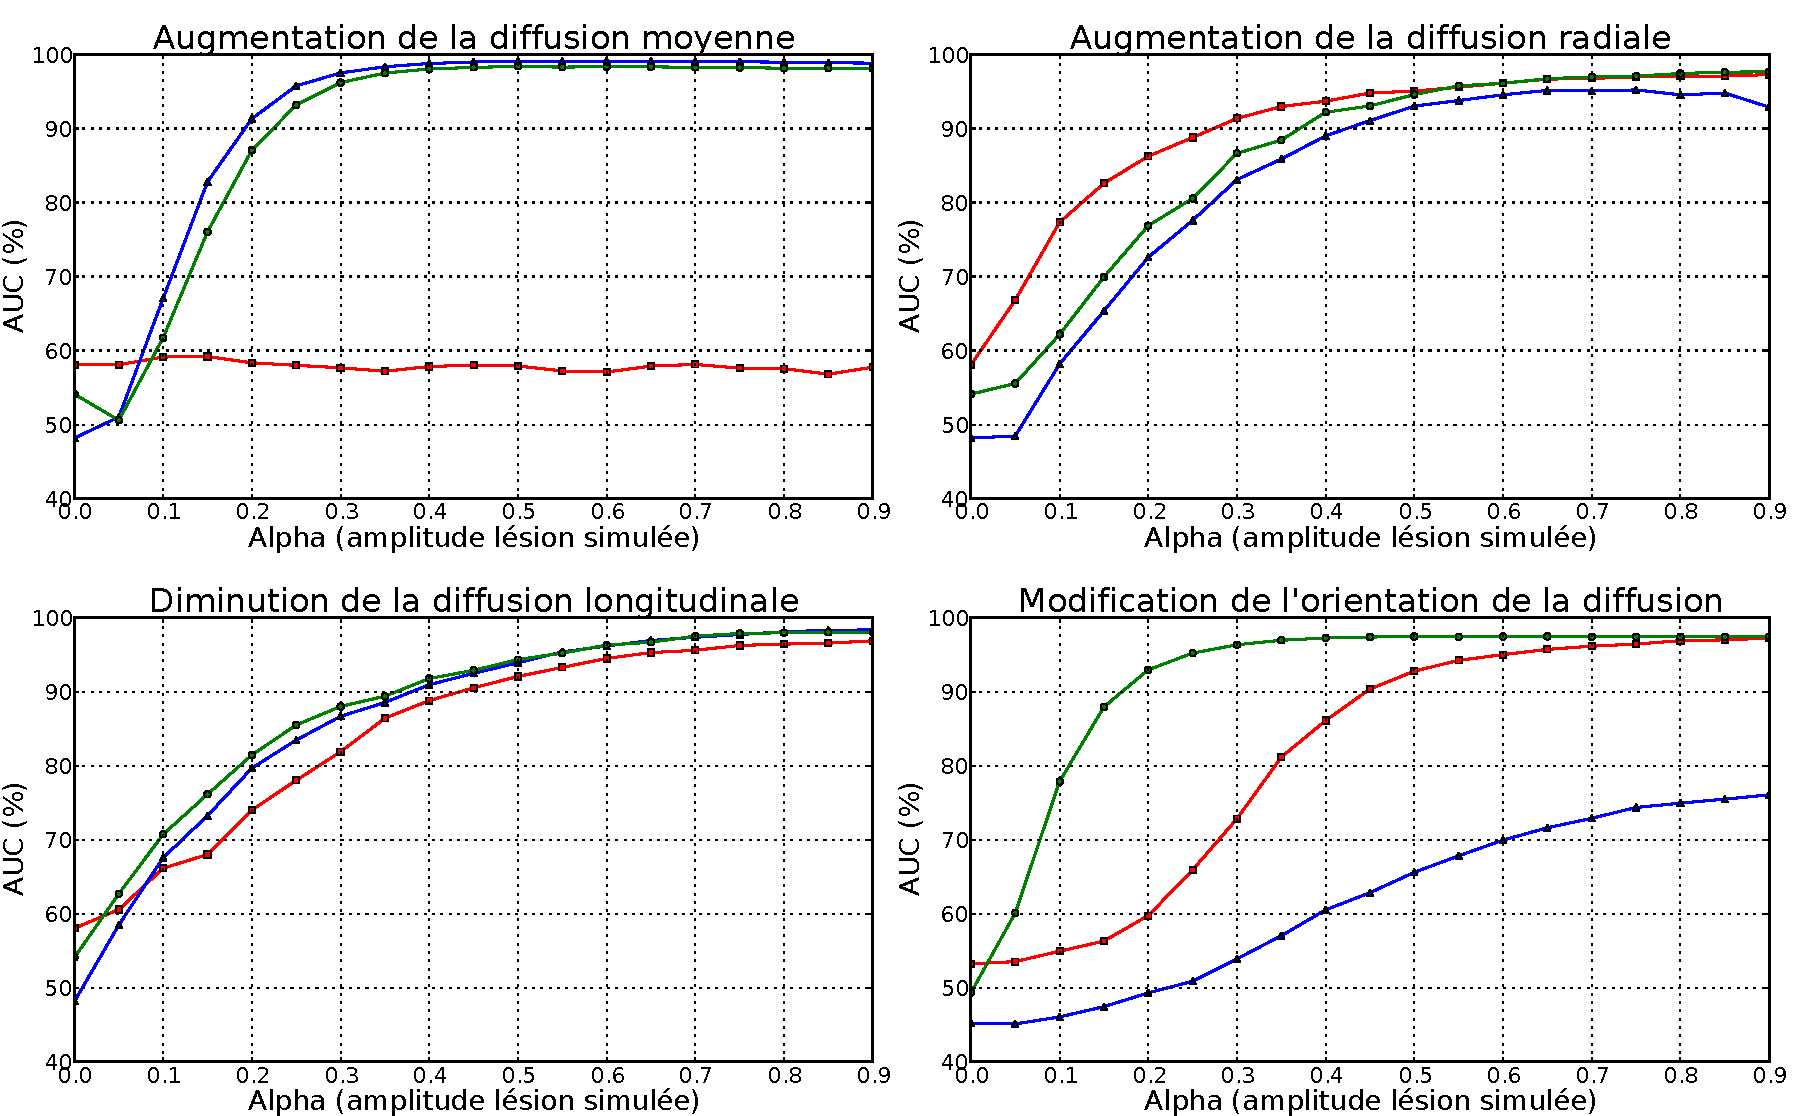
\includegraphics[width=1\textwidth]{Images/AUC_methods_gaussian8_fr.pdf}
    \caption{\label{fig:res_scalar} Comparaison entre les méthodes basées sur les indices scalaires ({\color{red} $\blacksquare$ = GLM-FA}, {\color{blue} $\blacktriangle$ = GLM-MD}) 
    et la méthode basée sur les tenseurs avec une métrique Euclidienne ({\color{green} $\bullet$ = GLM-DT}).}
\end{figure*}


\subsection{Discussion}
Une étude \cite{Whitcher2007} précédente a comparé des méthodes de compraison de groupes en ITD basées sur les indices scalaires avec certaines basées sur les tenseurs.
Dans cette étude, les auteurs ont considéré des métriques Euclidiennes et des métriques Log-Euclidiennes.
La différence principale de cette étude avec la notre est que les auteurs \cite{Whitcher2007} n'ont pas inclus de covariables telles que l'âge ou le genre dans leur analyse statistique.
De plus, ils n'ont pas pu inclure une comparaison avec des métriques Riemanienne telle que celle de \cite{Kim2014} car aucune n'était disponible en libre accès.
Ce qui est intéressant est que .

% A previous study has already compared scalar-based \textit{vs} several tensor-based methods for group comparison in DT-MRI \cite{Whitcher2007}. 
% They have considered both Euclidean and Log-Euclidean metrics.
% One of the main difference with our study is that the authors did not consider any covariates such as age or gender in their statistical analysis.
% They also did not have access to a Riemannian Manifold regression method such as \cite{Kim2014}.
The comparison between FA-based and tensor-based methods was also conducted on both simulated and real data.
The evaluation on simulated data highlights unsurprisingly that tensor-based methods are the only ones that are able to detect modification of diffusion orientation. 
The conclusion concerning the detection of FA alterations is more mitigated, since the FA-based approach slightly outperforms the tensor-based method relying on the Hoteling's $T^2$ test, 
but exhibits a lower statistical power than the tensor-based method relying on multivariate permutation test.
Our results are consistent with this paper since we also conclude that the tensor-based method is the only one that can efficiently detect every kinds of changes, 
although it can perform slightly worse than scalar-based methods for some particular changes 
(\textit{e.g.} FA-based method is the best performer to detect an augmentation of radial diffusion
and MD-based method is the best performer to detect an augmentation of mean diffusion).
Their conclusions on a cohort of patients with a history of migraine is also mitigated since both FA-based and tensor-based methods can detect
a cluster into the bank of the postcentral gyrus, but with a slightly greater spatial extent for the tensor-based method. 
This may be probably explained by a gain in statistical power allowed by the permutation test.

At the sight of our conclusions and the ones obtained by Whitcher \textit{et al.} \cite{Whitcher2007}, 
we can give the following recommendation to help the reader to choose between conducting a group study 
using either a scalar-based or a tensor-based method. 
If one has a strong \textit{a priori} about the kind of changes to detect (\textit{e.g.} a modification of the mean diffusivity), 
it is preferable to resort to the scalar-based approach on the appropriate scalar images (\textit{e.g.}  MD). This would be easier to implement and may lead to better performance.
If one has no prior on the expected changes, it would be preferable to use the tensor-based approach rather than performing several scalar-based analysis on different indices. 
By this way, it avoids the problem of multiple comparison (as compared to perform several tests on different indices) and lead to a unique detection map.
Nonetheless, using a tensor-based method would necessarily require a characterization step (section \chapref{Chapter6})
in order to help the physician or the neuroscientist in their interpretation.
Finally, one of the main added value of the tensor-based method is its ability to detect the modifications of diffusion orientation. 
However, this may be of limited interest in the context of voxelwise group comparison since most pathologies do not cause modifications of diffusion orientation in a consistent area across
a population. Modifications of orientation are generally observed in the vicinity of multiple sclerosis lesions or 
glioma and are generally related to the effect of oedema.
Consequently, this property may be more interesting for the follow-up of a given patient \cite{Grigis2012} than for group studies.


\section{Méthodes multi-informations \textit{vs} méthode GLM-DT}

\subsection{Informations d'hétéroscédasticité}
\begin{figure*}[t]
    \centering
    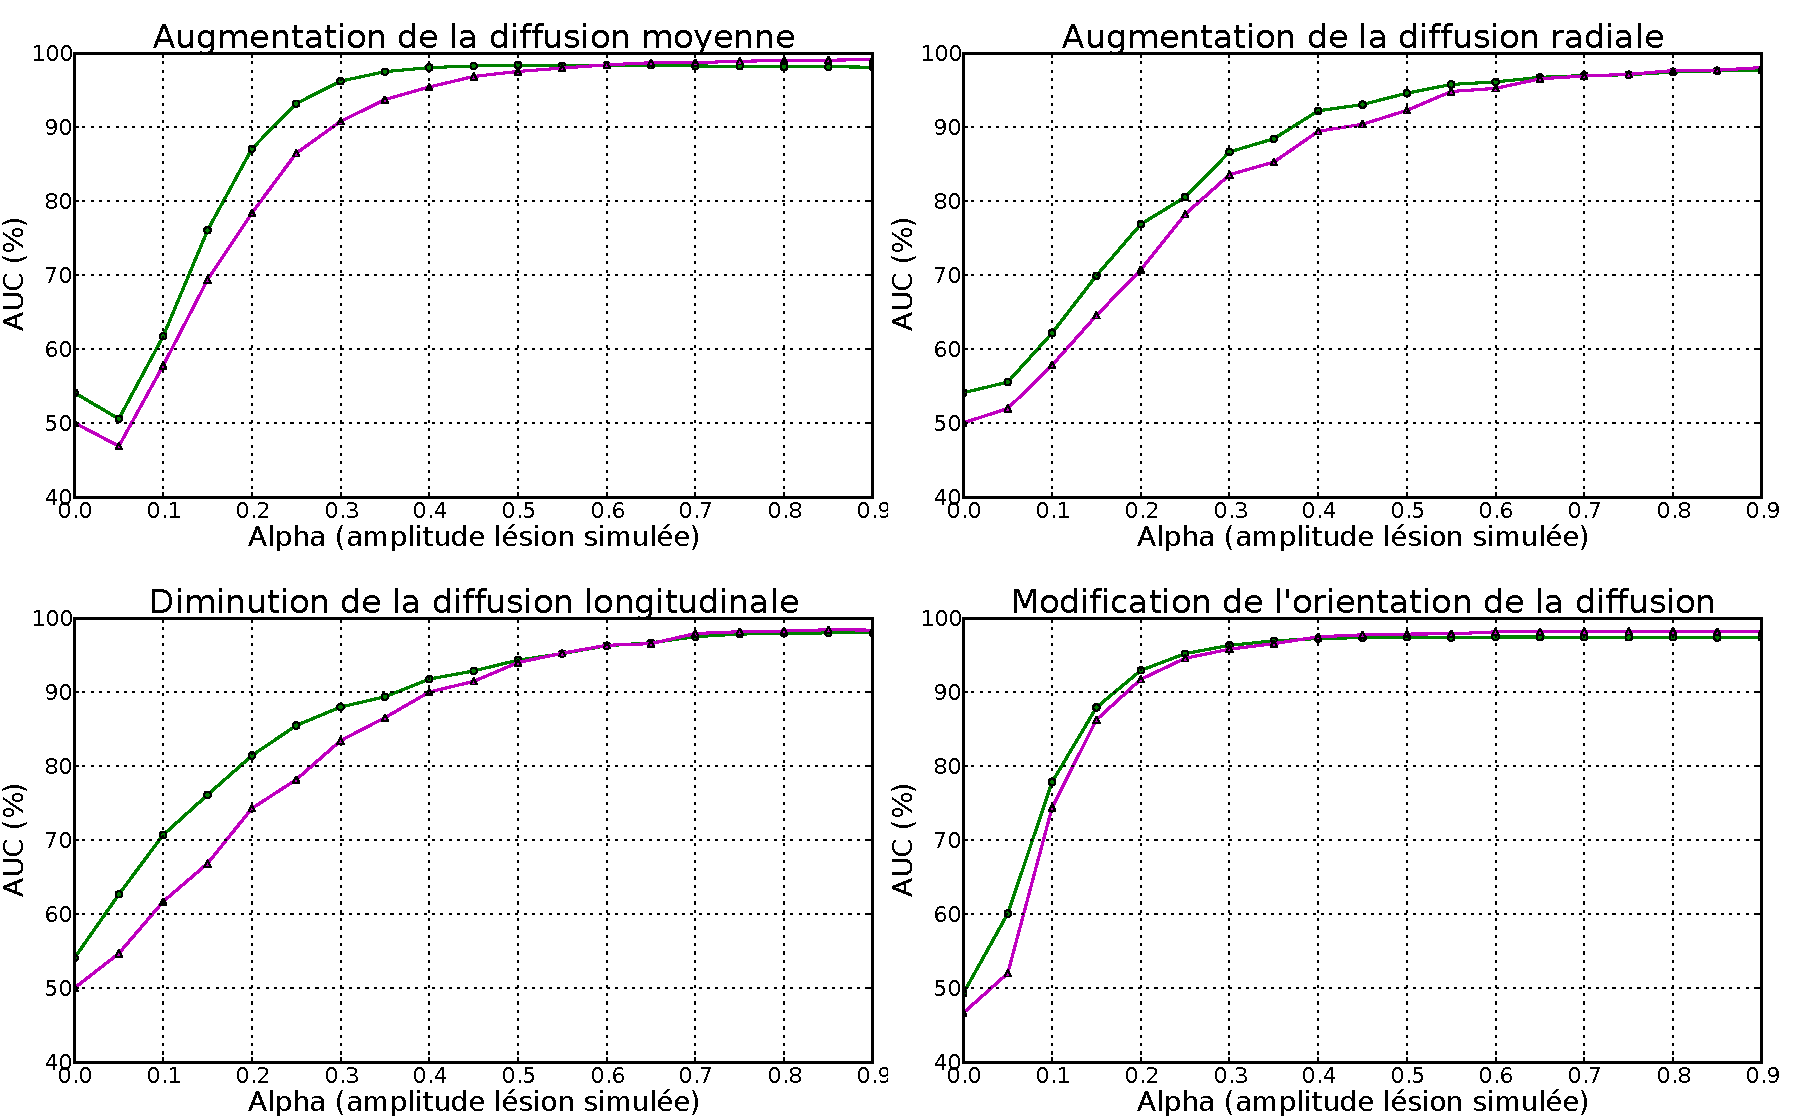
\includegraphics[width=1\textwidth]{Images/AUC_hetero_gaussian8_fr.pdf}
    \caption{\label{fig:res_hetero} Comparaison des méthodes basées sur les tenseurs dans un cadre Euclidien avec une hypothèse d'homoscédasticité sur les résidus ({\color{green} $\bullet$ = GLM-DT})
    et une hypothèse d'hétéroscédasticité ({\color{magenta} $\blacksquare$ = GLM-DT-H}).}
\end{figure*}

\subsection{Informations multi-échelles}
\begin{figure*}[t]
    \centering
    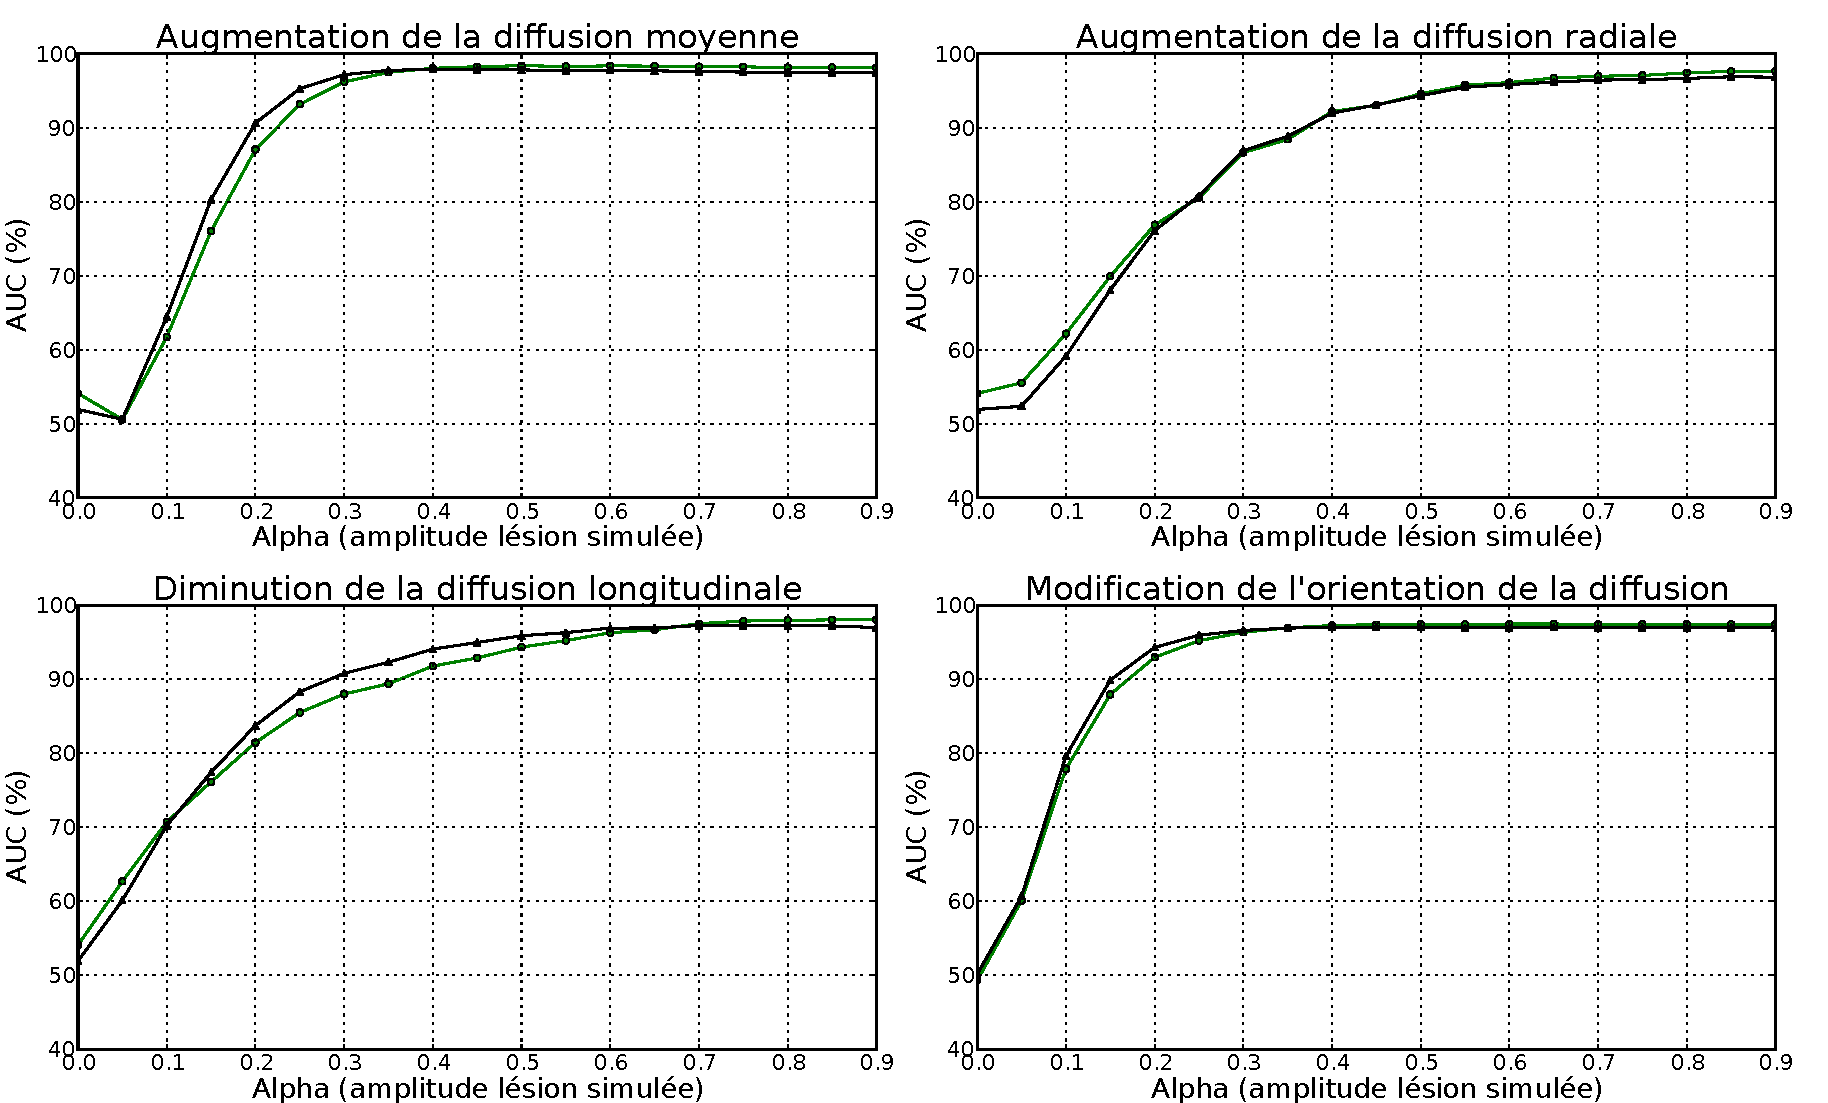
\includegraphics[width=1\textwidth]{Images/AUC_multiscale_gaussian8_fr.pdf}
    \caption{\label{fig:res_multiscale} Comparaison dans un cadre Euclidien entre la méthode basée sur les tenseurs ({\color{green} $\bullet$ = GLM-DT})
    et une méthode basée sur les tenseurs utilisant des informations multi-échelle ({\color{black} $\blacksquare$ = GLM-DT-fusion}).}
\end{figure*}

\section{Validation de la méthode de caractérisation}

Le \tabref{tab:res_carac} présente les résultats de la méthode caractérisation appliquée à trois groupes de données simulées : $\alpha=0.2$, $\alpha=0.5$, $\alpha=0.9$.
Pour chaque type de lésion et chaque amplitude, la liste des informations statistiques est affichée pour tous les agrégats détectés. 
Par exemple, il y a 2 agrégats détectés par la méthode \textit{GLM-DT} pour une simulation d'augmentation de diffusion moyenne avec une amplitude de $\alpha=0.2$.
Seuls les agrégats qui recouvrent d'au moins 1 voxel la vérité terrain (Vrais Positifs), sont présentés dans le \tabref{tab:res_carac}.

Les résultats montrent que chaque lésions simulées est correctement caractérisée par la méthode
(d'après le tableau d'interprétation géométrique donné en).
Il y a une exception pour l'augmentation de la diffusion moyenne avec une amplitude de $\alpha=0.2$ 
où le second agrégat est classé comme une augmentation de la diffusion radiale.

\begin{table}
    \centering
    \begin{tabular}{|D{0.5\textwidth}||cc|cc|cc|}
	\hline
	\multirow{2}{*}{\diagbox{\textbf{Lésion simulée}}{$\alpha$}} & \multicolumn{2}{c}{$0.2$} & \multicolumn{2}{c}{$0.5$} & \multicolumn{2}{c|}{$0.9$} \tabularnewline
	 & \textbf{MD} & \textbf{FA} & \textbf{MD} & \textbf{FA} & \textbf{MD} & \textbf{FA} \tabularnewline
	\hline
	\multirow{2}{*}{augmentation de la diffusion moyenne} & $+$ & n.s. & \multirow{2}{*}{$+$} & \multirow{2}{*}{n.s.} & \multirow{2}{*}{$+$} & \multirow{2}{*}{n.s.} \tabularnewline
	 & $+$ & $-$ & & & & \tabularnewline
	\hline
	\multirow{3}{*}{augmentation de la diffusion radiale} & \multirow{2}{*}{$+$} & \multirow{2}{*}{$-$} & $+$ & $-$ & \multirow{2}{*}{$+$} & \multirow{2}{*}{$-$} \tabularnewline
	 & & & $+$ & $-$ & & \tabularnewline
	 & $+$ & $-$ & $+$ & $-$ & $+$ & $-$ \tabularnewline
	\hline
	\multirow{2}{*}{diminution de la diffusion longitudinale} & $-$ & $-$ & \multirow{2}{*}{$-$} & \multirow{2}{*}{$-$} & \multirow{2}{*}{$-$} & \multirow{2}{*}{$-$} \tabularnewline
	 & $-$ & $-$ & & & & \tabularnewline
	 \hline
	\multirow{2}{*}{modification de l'orientation de la diffusion} & n.s. & n.s. & \multirow{2}{*}{n.s.} & \multirow{2}{*}{n.s.} & \multirow{2}{*}{n.s.} & \multirow{2}{*}{n.s.}\tabularnewline
	 & n.s. & n.s. & & & & \tabularnewline
        \hline
    \end{tabular}
    \caption{\label{tab:res_carac} Résultats de la méthode de caractérisation pour la méthode \textit{GLM-DT} (seuil statistique $p_{FDR}=0.05$ et seuil $N_c=10$).
    (Légende: $+=$ augmentation significative, $-=$ diminution significative, $n.s.=$ non significatif)}
\end{table}





